\section{Gaussian models}
\subsection{Uncorrelated does not imply independent}
Let $X \sim U(-1,1)$ and $Y = X^2$. Clearly $Y$ is dependent on $X$ (in fact, $Y$ is uniquely determined by X). However, $\mathrm{cov}[X,Y] = \mathbb{E}[XY]-\mathbb{E}[X]\mathbb{E}[Y] = 0$ and so $\rho(X,Y)=0$, i.e. $X$ and $Y$ are uncorrelated.

\subsection{Uncorrelated and Gaussian does not imply independent unless \textit{jointly} Gaussian}
Let $X \sim \mathcal{N}(0,1)$ and $Y=WX$, where $p(W=-1)=p(W=1)=0.5$. It is clear that $X$ and $Y$ are not independent, since $Y$ is a function of $X$.\\\\
a. $p_Y(y) = \mathbb{P}(Y=y) = \mathbb{P}(W=1,X=y) + \mathbb{P}(W=-1,X=-y) = 0.5p_X(y) + 0.5p_X(-y) = p_X(y)$ due to symmetry. So $Y \sim \mathcal{N}(0,1)$.\\\\
b. But $\mathrm{cov}[X,Y] = \mathbb{E}[XY] - \mathbb{E}[X]\mathbb{E}[Y] = \mathbb{E}_W[\mathbb{E}_{X,Y}[XY|W]] - \mathbb{E}_X[X]\mathbb{E}_Y[Y] = 0.5\mathbb{E}[X^2] + 0.5\mathbb{E}[-X^2] - 0 = 0$, so $X$ and $Y$ are uncorrelated.\\\\
Note that in the jointly Gaussian case, we can factorise the joint distribution (implying independence) if the covariance matrix is diagonal (implying uncorrelated variables).

\subsection{Correlation coefficient is between -1 and +1}
We note that the covariance specifies an inner product, as it is symmetric, positive definite and linear (in the first argument). Thus by Cauchy-Schwarz, we have
\begin{align*}
|\mathrm{cov}(X,Y)| &\leq \mathrm{cov}(X,X) \cdot \mathrm{cov}(Y,Y)\\
&= \sigma_X\sigma_Y\\
|\rho(X,Y)| &= \frac{|\mathrm{cov}(X,Y)|}{\sigma_X\sigma_Y}\\
&\leq 1.
\end{align*}

\subsection{Correlation coefficient for linearly related variables is $\pm1$}
If $Y=aX+b$, then
\begin{align*}
\sigma_Y^2 &= \mathbb{E}[Y^2] - \mu_Y^2\\
&= \mathbb{E}[(aX+b)^2] - (a\mu_X+b)^2\\
&= a^2(\sigma_X^2+\mu_X^2) + 2ab\mu_X + b^2 - (a\mu_X+b)^2\\
&= a^2\sigma_X^2\\
\mathrm{cov}(X,Y) &= \mathbb{E}[X(aX+b)] - \mu_X(a\mu_X+b)\\
&= a(\sigma_X^2+\mu_X^2) + b\mu_X - \mu_X(a\mu_X+b)\\
&= a\sigma_X^2\\
\rho(X,Y) &= \frac{\mathrm{cov}(X,Y)}{\sigma_X\sigma_Y}\\
&= \frac{a\sigma_X^2}{\sigma_X\sqrt{a^2\sigma_X^2}}\\
&= \frac{a}{|a|}.
\end{align*}

\subsection{Normalisation constant for a multivariate Gaussian}
Since $\bm{\Sigma}$ is symmetric, it is diagonalisable such that $\bm{\Sigma} = \bm{P}\bm{D}\bm{P}^T$ with $\bm{D} = \mathrm{diag}(\lambda_1,\dots,\lambda_d)$, $\bm{P}$ orthogonal. Thus
\begin{align*}
&\int \exp(-\frac{1}{2} (\bm{x}-\bm{\mu})^T \bm{\Sigma}^{-1} (\bm{x}-\bm{\mu})) \diff\bm{x}\\
=\ &\int \exp(-\frac{1}{2} (\bm{x}-\bm{\mu})^T \bm{P}\bm{D}^{-1}\bm{P}^T (\bm{x}-\bm{\mu})) \diff\bm{x}\\
=\ &\int \exp(-\frac{1}{2} (\bm{P}^T\bm{x}-\bm{P}^T\bm{\mu})^T \bm{D}^{-1} (\bm{P}^T\bm{x}-\bm{P}^T\bm{\mu})) \diff\bm{x}\\
=\ &\int \exp(-\frac{1}{2} (\bm{y}-\bm{\mu})^T \bm{D}^{-1} (\bm{y}-\bm{\mu})) \diff\bm{y}\\
=\ &\prod_{i=1}^{d} \int \exp(-\frac{1}{2} (y_i-\mu_i)\lambda_i^{-1}(y_i-\mu_i)) \diff y_i\\
=\ &\prod_{i=1}^{d} \sqrt{2\pi\lambda_i}\\
=\ &(2\pi)^{d/2}|\bm\Sigma|^{1/2}
\end{align*}
where we use the fact that $|\bm{P}| = 1$ in the change of variables to $\bm{y} = \bm{P}^T\bm{x}$.

\subsection{Bivariate Gaussian}
Let $\bm{x} \sim \mathcal{N}(\bm{\mu}, \bm{\Sigma})$, where $\bm{x} \in \mathbb{R}^2$ and
\begin{equation*}
\bm{\Sigma} = \begin{pmatrix} \sigma_1^2 & \rho\sigma_1\sigma_2 \\ \rho\sigma_1\sigma_2 & \sigma_2^2 \end{pmatrix}
\end{equation*}
where $\rho$ is the correlation coefficient. Thus $|\bm{\Sigma}| = (1-\rho^2)\sigma_1^2\sigma_2^2$, and the pdf
\begin{align*}
p(x_1,x_2) &= \frac{1}{2\pi\sqrt{|\bm{\Sigma}|}} \exp(-\frac{1}{2} (\bm{x}-\bm{\mu})^T \bm{\Sigma}^{-1} (\bm{x}-\bm{\mu}))\\
&= \frac{1}{2\pi\sqrt{|\bm{\Sigma}|}} \exp\left( -\frac{1}{2|\bm{\Sigma}|} \begin{pmatrix}x_1-\mu_1\\x_2-\mu_2\end{pmatrix}^T \begin{pmatrix}\sigma_2^2&-\rho\sigma_1\sigma_2\\-\rho\sigma_1\sigma_2&\sigma_1^2\end{pmatrix} \begin{pmatrix}x_1-\mu_1\\x_2-\mu_2\end{pmatrix} \right)
%&= \frac{1}{2\pi\sqrt{|\bm{\Sigma}|}} \exp\left( -\frac{1}{2(1-\rho^2)} \left[ \frac{(x_1-\mu_1)^2}{\sigma_1^2} - \frac{2\rho(x_1-\mu_1)(x_2-\mu_2)}{\sigma_1\sigma_2} + \frac{(\sigma_2-\mu_2)^2}{\sigma_2^2} \right] \right)
\end{align*}
which expands to give the desired expression.

\subsection{Conditioning a bivariate Gaussian}
Consider a bivariate Gaussian distribution $p(x_1,x_2) = \mathcal{N}(\bm{x}|\bm{\mu},\bm{\Sigma})$, where
\begin{gather*}
\bm{\Sigma} = \begin{pmatrix}\sigma_1^2&\sigma_{12}\\\sigma_{21}&\sigma_2^2\end{pmatrix} = \sigma_1\sigma_2 \begin{pmatrix}\frac{\sigma_1}{\sigma_2}&\rho\\\rho&\frac{\sigma_2}{\sigma_1}\end{pmatrix},\ \rho = \frac{\sigma_{12}}{\sigma_1\sigma_2}
\end{gather*}
a.
\begin{align*}
p(x_2|x_1) =&\ \frac{p(x_1,x_2)}{p(x_1)}\\
=&\ \frac{1}{\sqrt{2\pi(1-\rho^2)}\sigma_2} \exp\bigg( -\frac{1}{2(1-\rho^2)}\bigg[ \frac{(x_1-\mu_1)^2}{\sigma_1^2} + \frac{(x_2-\mu_2)^2}{\sigma_2^2}\\
&\ - 2\rho\frac{(x_1-\mu_1)}{\sigma_1}\frac{(x_2-\mu_2)}{\sigma_2} \bigg] + \frac{(x_1-\mu_1)^2}{2\sigma_1^2} \bigg)\\
=&\ \frac{1}{\sqrt{2\pi(1-\rho^2)}\sigma_2} \exp\bigg( -\frac{1}{2(1-\rho^2)}\bigg[ \rho^2\frac{(x_1-\mu_1)^2}{\sigma_1^2} + \frac{(x_2-\mu_2)^2}{\sigma_2^2}\\
&\ - 2\rho\frac{(x_1-\mu_1)}{\sigma_1}\frac{(x_2-\mu_2)}{\sigma_2} \bigg] \bigg)\\
=&\ \frac{1}{\sqrt{2\pi(1-\rho^2)}\sigma_2} \exp\bigg( -\frac{1}{2(1-\rho^2)}\bigg[ \rho\frac{(x_1-\mu_1)}{\sigma_1} - \frac{(x_2-\mu_2)}{\sigma_2} \bigg]^2 \bigg)\\
=&\ \frac{1}{\sqrt{2\pi(1-\rho^2)}\sigma_2} \exp\bigg( -\frac{1}{2(1-\rho^2)\sigma_2^2}\bigg[ x_2 - (\mu_2 + \rho\frac{\sigma_2}{\sigma_1}(x_1-\mu_1)) \bigg]^2 \bigg)\\
=&\ \mathcal{N}(x_2|\mu_2 + \rho\frac{\sigma_2}{\sigma_1}(x_1-\mu_1),(1-\rho^2)\sigma_2^2)
\end{align*}
which fits with the general results given in the book (4.69).\\\\
b. With $\sigma_1=\sigma_2=1$, we have $p(x_2|x_1) = \mathcal{N}(x_2|\mu_2+\sigma_{12}(x_1-\mu_1),1-\sigma_{12}^2)$. We see that knowing $x_1$ can decrease the variance of $x_2$ and translate its distribution, if the two variables are correlated.

\subsection{Whitening vs standardising}
\begin{figure}[h]
\centering
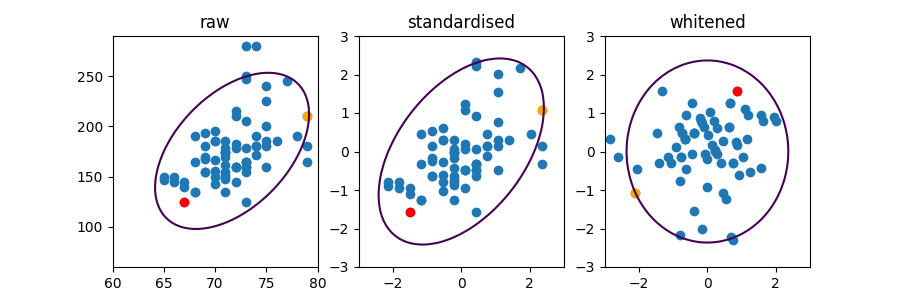
\includegraphics[width=\linewidth]{4-gaussian-models/48-whiten-stdise}
\end{figure}
